\documentclass[12pt]{report}
\usepackage{import}
\usepackage{preamble}

\title{Evaluating Utility of Vocabulary to Language Learners}
\author{Leonard Paál\\Hochschule Karlsruhe\\Supervising professor: Jannik Strötgen\\Additional supervision by: John Blake (University of Aizu)}
\date{May 2025}

\begin{document}

\maketitle

Hiermit erkläre ich, dass ich die vorliegende Arbeit selbstständig und ohne fremde Hilfe verfasst und keine anderen Hilfsmittel als die angegebenen verwendet habe.
Insbesondere versichere ich, dass ich alle wörtlichen und sinngemäßen Übernahmen aus anderen Werken als solche kenntlich gemacht habe.
\\

Aizuwakamatsu, 10. Mai 2025

\selectlanguage{ngerman}
\begin{abstract}
	The Erstellung von Vokabellisten ist ein essenzieller Bestandteil des Sprachenlernens.
	Aktuelle Methoden zur Auswahl von Vokabular basieren entweder auf dem reinen Zählen von Wörtern, oder werden durch Experten erstellt, was einen arbeitsintensiven Prozess darstellt.
	Diese Arbeit präsentiert ein Framework, um möglichst nützliche Vokabellisten automatisch mithilfe von AI- und XAI-Methoden zur erstellen, sowie Vokabellisten automatisch auszuwerten, und benutzt hierfür frei zugängliche, nichtkommerzielle Korpora.
	Die vorgestellte Implementierung des Ansatzes unterstützt geschätzt die automatische Erstellung und Auswertung von Vokabellisten in neun Sprachen mit dem Filtern von Namen, und ca. vierzig Sprachen ohne Filtern von Namen.
	Unsere Experimente legen nahe, dass die von unseren Methoden generierten Vokabelliste Sprachlernenden schneller zu sprachlicher Kompetenz in den angestrebten Kontexten verhelfen als Ansätze, die auf reiner Wortfrequenz basieren.
\end{abstract}

\selectlanguage{english}
\begin{abstract}
	Compiling lists of vocabulary is an essential part in language teaching.
	Current methods used to select vocabulary rely either on pure word counting, or on the manual selection of vocabulary by experts, which is a labor-intensive process.
	This work suggests a framework for automatically compiling lists of vocabulary that are more useful than those produced by frequency-based approaches, using public and freely accessible corpora and AI models, as well as evaluating said lists.
	We describe the implementation of the framework in detail.
	Our implementation supports approximately 9 languages with name filtering, and 40 languages without name filtering, though evaluation was only performed on English data.
	The evaluation suggests that our compiled lists are more useful for understanding the context they were compiled for than those produced by word counting, especially for narrow contexts such as single subtitles and articles.
\end{abstract}


\clearpage
\tableofcontents
\clearpage

\chapter{Introduction} \label{ch:intro}
\section{Motivation}
\subsection{Role of vocabulary in language acquisition}
Learning a second language involves many different skills, often categorized into listening, reading, speaking, and writing.
Another categorization may be vocabulary, grammatical skills, the ability to understand known words in various accents, understanding language when spoken at a fast speed.
One skill that is required for any of these if the knowledge of vocabulary in the target language.
A person with basic grammatical skills but no vocabulary has no ability to express themselves or understand anything which they hear around them.
On the other hand, a person familiar with rudimentary vocabulary but no grammatical knowledge may struggle with understanding complex sentences and sound unnatural when speaking, but can at least make sense of short phrases and express themselves.
Thus, basic knowledge of vocabulary is clearly one of the most essential skills for using a language.
This raises the question of which vocabulary should be learned first when starting out on the journey of language acquisition.


\subsection{Context-specific language learning}
Learners of languages are typically interested in one or more specific aspects of the language.
There is no such thing as an unbiased corpus than can fit every use case.
Decisions must be made how much focus is given to everyday conversation, academic writing, writing pertaining to business like job applications etc.
Many textbooks group vocabulary by topic, with a new topic being introduced with each lesson that student should ideally be able to converse in after completing the lesson.
However, this way of introducing vocabulary has several shortcomings:
\begin{itemize}
	\item Students spend time learning specific terms about the topic in one lesson while not learning even general vocabulary in other topics until much later.
	\item Knowing the words from previous lessons becomes a prerequisite for the more advanced material, especially because the terms from earlier lessons are used in example sentences for grammar.
	      Thus, learners interested in learning the use of the language in one context will have a hard time of skipping earlier, less pertinent lessons to them.
\end{itemize}

Since the advent of computer-aided natural language processing, methods have been suggested to computationally identify useful words:
Nation and Waring propose in an 1997 study \cite{nationVocabularySizeText1997} that the frequency with which a word appears in the target language should be used a metric for its importance to the learner, or utility, and thus teaching high-frequency words should be the focus when teaching beginners.
However, focusing on maximum-frequency words to achieve text coverage (e.g., knowledge of 90\% of words in a text) may not be as useful as one might at first think, as the most frequent words tend to be generic terms like “but”, “from”, “time”, “world” etc.
Knowing only these words is not sufficient for comprehending most texts.

The TF-IDF metric \cite{qaiserTextMiningUse2018} is often employed for finding the keywords in a document and thus a proxy for how important a word is for the overall meaning of the document.
It essentially is a frequency normalized against a larger, background corpus and expressed whether the usage frequency in the document is unusual.
Using TF-IDF as a measure for utility of a word in a given context is possible, but it suppresses words that may be generally useful.

Thus, there is a need for further exploration as to how word utility can be calculated, using modern NLP methods involving artificial intelligence where necessary.
Put more simply, this question may be reduced to:

\textbf{What order or words, when learned, gives the learner the best set of words to understand and communicate in the language as quickly as possible?}

\subsection{Examples of contexts and words}
Some examples for contexts that could be interesting to language learners include:

\begin{itemize}
	\item Reading Wikipedia articles about a specific field (computer science, literature, biographies)
	\item Watching movies
	\item Travel to a country where the target language is spoken
	\item Doing business with a company from a country where the target language is spoken
	\item Cultural exploration (literature, religion)
	\item Finding friends from other countries
\end{itemize}

The different contexts for which learners might be motivated to learn a language differ in how easily corpora can be obtained about to mine patterns from. Movie subtitles and Wikipedia articles are easily obtained from sites such as opensubtitles.org and wikipedia.org. The words that might be relevant for travel are not as easily obtained: One might imagine an ideal scenario to collect data, in which a statistically relevant group of people travelling to the destination to be examined are randomly selected and equipped with microphones and cameras before the travel. During travel, one could record their conversations, conversations with people around them, and materials they attempt to read to navigate their journey such as train schedules, descriptions of tours, restaurant menus, street signs, etc. Lacking the funds to conduct an experiment for every possible language, this paper is interested in finding a methodology to obtain data from readily available corpora and websites online that extracts relevant vocabulary from the source texts.
Depending on the context, we can think about which of the following English words might be likely to appear frequently in the texts:

\begin{itemize}
	\item Convert
	\item Cash
	\item Hug
	\item Dammit
	\item Y'all
	\item From
	\item Nineen eighty four
	\item Married
\end{itemize}

To examine a few examples: Words like “convert” occur frequently when looking at Wikipedia articles \footnote{see "Wikipedia" corpus 2016, drawn from one million lines on https://wortschatz.uni-leipzig.de/en/download/English}. “cash” is likely to be useful for travelers, but in most other contexts, it would not be as relevant. “Y’all” is almost never used in formal writing but used abundantly in everyday speech in the southern United Stated of America and South Africa. “From”, meanwhile, will be likely to be one of the most frequently used words regardless of context.

\section{Background}
\subsection{Requirements for calculating word utility from existing data}

\begin{description}
	\item [Large word corpora in many languages]
	\item [Hardware capabilities]
	\item [Software is able to process text on semantic level]
	      Text processing software and tools have existed since the 1980s, however before the advent of neural networks and other artificial intelligence methods, their capabilities were mostly bereft of any semantic understanding of the text processed: Using exclusively manually crated tools, it is possible to create a program which recognizes that \textit{table} and \textit{tables} derive from the same word, but much harder to recognize that there is any connection whatsoever between \textit{table} and \textit{chair}. The language processing capabilities of any human dwarf those of these early tools.
\end{description}

\subsection{Developments in Natural Language Processing}
\begin{description}
	\item [Sophisticated tokenizers]
	\item [Wordnets]
	\item [Neural networks trained in NLP tasks]
	\item [Explainable AI]
\end{description}

This paper aims to exploit these significant developments to gain insights into which words can provide second language learners with the most utility.

\section{Method of this paper}
It is evident that recent tools based on Artificial Intelligence are much better-equipped for many tasks in the realm of Natural Language Processing than rule-based tools.
At the same time, it is less clear how exactly these networks achieve the results they do.
Fortunately, there is a branch in the field of Artificial Intelligence called Explainable Artificial Intelligence which aims at explaining the outputs of AI models.
Thus, it may be possible to harness the evident intelligence off AI models to simulate a human, to find out which words have the largest impact on the model's performance.

\subsection{Word extraction methods}
The approaches for approximating utility with an automatically computable metric which this works aims to compare include:
\subsubsection{Traditional}
\begin{description}
	\item [Raw frequency of words in corpus]
	      A simple ordering of words by how often they appear in a corpus.
		\item[Frequency with stopwords filtered out]
			The same as frequency, but filtering out known stopwords from the resulting lists.
	\item [TF-IDF]
	      How often the words appear in a target corpus but divided by their frequency in a more generic corpus.
	      This metric is typically used to employ the most relevant words in documents for identifying keywords that express best its core topic.
\end{description}
\subsubsection{AI-simulated learner}
\begin{description}
	\item [Performance difference of AI for NLP tasks]
	      Here, a Large Language Model (LLM) or a more specific language processing model is made to run NLP tasks such as text summarization, sentiment detection or question-answering.
	      To find out which words help the AI model the most in performing its tasks, words are methodically omitted from texts and the AI’s performance is recorded.
	      This metric attempts to approximate utility by finding words which, when missing, cause the greatest performance loss in the NLP tasks.
		  Evaluation metrics like Shapley values \cite{wangShapleyExplanationNetworks2021} may be used to measure the impact of missing words
	\item [Transformer attention]
		The transformer architecture is based on a mechanism called \textit{self-attention}.
		It allocates the neural network's processing to important parts of the input and thus provides some degree of explainability "out of the box".

	\item [Difference in internal vector representation for AI reading text]
	      This approach words similarly to the above involving an AI model, but instead of measuring the changes in the quality of its output, it measures how much changing the input to the model changes its the internal vector state: AI stores data in vector format, and when performing NLP tasks on texts, there is an internal vector representation.
	      By using various distance metrics, it may be possible to find out which words have the greatest impact on the model’s understanding of a text.
	      Most of these approaches can be done both for individual words and word sequences (n-grams).
	      While individual words are the easiest to examine, sometimes n-grams are insightful for finding sequences of words whose meaning is more than the sum of their parts (idioms and collocations) and which therefore must be learned in separately from their constituents (meaningful English n-grams include e.g. “kick the bucket”, “such that”, “such as”).

	      This also raises the question of what is considered a “word”.
	      A phrase like “such as” can be considered two words if the definition of a word is simply “something separated by a space” or one word if the definition is “a phrase whose meaning cannot be arrived at trivially from knowing the definition of its parts”.
	      In Natural Language Processing, tokenizers break down texts into words, but they typically use the first definition for a word in the case of English.
	      Many non-European language do not use spaces in their spelling (e.g. Japanese, Mandarin Chinese) or use spaces to separate a different unit of text (syllables in Vietnamese, sentences in Thai), making this definition of a word unpractical.
	      In most languages, words can appear in various different forms: Verbs in Spanish are conjugated according to the time and originator of an action, Nouns in German are declined depending on their number and grammatical case.
	      This adds another variable for compiling word lists: Whether the list should consider any different combination of letters as a different word, or whether different forms of the same headword should be viewed as only one word.
\end{description}

Key technologies employed include therefore:
\begin{itemize}
	\item Tokenizers
	\item Lemmatizers
	\item Translators
	\item AI models to perform NLP tasks
\end{itemize}


\chapter{Background} \label{ch:background}
\section{Current teaching of languages}
 [Short overview what percentage is taught via classrooms/learning apps/textbooks]
 [I want to develop a method that helps educators (and active students) to select relevant vocabulary.]

\section{Basic concepts of Natural Language Processing}
 [basic concepts, and why they matter to this work.
  I will add anything that that the target audience is either not familiar with, or where the function in my method is not obvious]

\begin{description}
	\item [AI model] Container of functional knowledge, in this case linguistic.
	\item [General NLP tasks] a) Way for AI model to engage with language, b) Test of language ability.
	\item [Explainable AI] Extraction of knowledge from AI model.
	\item [Transformer Attention mechanism] Way of finding patterns in functional knowledge of some AI models.
	\item [Tokenizer] To split continuous text into distinct words, which we can make statistics from, mask in text etc.
\end{description}

This paper aims to exploit these significant developments to gain insights into which words can provide second language learners with the most utility.

\section{Definitions of terms}
 [Definition of "utility" of vocabulary]

\section{State of the Art (of vocabulary selection)}
\subsection{Non-computational methods}
How is vocabulary order selected by current language teaching tools:
Not context-specific in most cases
offers only one order,
investigate if there are any automatic approaches besides frequency]

[can present methods for extracting useful words from text]
can be similar in either method or goal.
goal is finding useful words for language learning
method is extracting important words from text via XAI

\subsection{Computational methods}
These methods generate vocabulary lists by using corpora and computer-aided language processing to compile vocabulary lists.
These are closer to the method I will

\begin{description}
	\item [Raw frequency of words in corpus]
	      A simple ordering of words by how often they appear in a corpus.
	\item [Frequency with stopwords filtered out]
	      The same as frequency, but filtering out known stopwords from the resulting lists.
	\item [TF-IDF]
	      How often the words appear in a target document but divided by their frequency in a more generic corpus.
	      This metric is typically used to employ the most relevant words in documents for identifying keywords that express best its core topic.
\end{description}

\subsection{Issues with current methods}
Current methods do not exploit recent developments in AI technology and thus suffer from several shortcomings:
In general, all of them essentially only count words without taking into account their relationship between each other:

Frequency: The most frequent words in texts are often words that carry little meaning by themselves, such as "a", "the", "of" in English.
While these may appear in many texts, they are not useful in determining their meaning.
TF-IDF: This metric has been used successfully to find the words that give the best hints at a text's topic.
However, it does not take into account and semantic relationships between the words in a text.
Thus, learning words by aggregating TF-IDFs on multiple texts may aid in identifying the topic of texts, but not at finding out what the message conveyed about the topic is.
"not" is a highly frequent word in English and thus will have a low TF-IDF score in most documents. But it is essential to know, as it can completely invert the meaning of a sentence.


\chapter{Approach} \label{ch:approach}
This chapter describes in detail our approach for word utility evaluation to fulfill the goal stated in Section \ref{sec:statement-of-goal}.
The problem is first put formally by putting the terms of word utility and vocabulary list efficiency into mathematical objects in Section \ref{sec:formal-problem-statement}.
We then describe a hypothetical experiment that could be performed to evaluate word utility using human feedback in Section \ref{sec:human-efficiency-testing}.
After pointing out the unfeasibility of such a testing method, we suggest ways to perform the experiment with AI models instead of humans as the test subject in Section \ref{sec:experimental-setup-with-ai}, using the technological building blocks referred to previously in Chapter \ref{ch:background}.

With a method for utility evaluation established, we then point out why it is in itself not yet sufficient for actually generating useful lists of vocabulary that a human learner could utilize in Section \ref{sec:eval-vs-creation}.
To solve this final problem, \ref{sec:list-generation} puts forward a general approach for list generation.

\section{Formal Problem Statement} \label{sec:formal-problem-statement}

To repeat the core statement from Section \ref{sec:statement-of-goal}:
The aim of this work is to create computational approaches to find words that have the maximum \textit{utility} given a particular \textit{language context} by means of \textit{proxy tasks}.

Keeping in mind that this is done in order to sort words into vocabulary lists that can be used by language learners, we can conclude that the output of a proposed solution to this problem would be an ordered list of words.
If this word list is ordered by descending word utility, we might speak of a \textit{maximally efficient} vocabulary list.
We could also put a number on \textit{any} list of words which measures how efficient a vocabulary list is to gain understanding in a given linguistic context.
A list should be evaluated as more efficient if useful words appear at the top of the list, and less efficient if less useful words are at the top, since such an order implies that someone learning the words in that order would not gain understanding at the highest possible rate.

We can subdivide the overarching goal of word utility evaluation into three related, but not quite equivalent sub-goals:
\begin{itemize}
	\item Evaluating the utility of a single word.
	\item Evaluating the efficiency of a list of words to learn.
	\item Generating maximally efficient lists of words to learn.
\end{itemize}

This section puts utility and efficiency into mathematical terms, to provide a clearer explanation of the variables involved in these tasks and their relationship.

\subsection{Proxy Task}
Since utility is defined in terms of language ability, we first need a way to put a number on the language ability of a test subject. This is done by means of a proxy task: We can imagine a human test subject taking a language exam as a proxy task to find out their language ability:

\begin{align*}
	t: \text{Human} & \to [0, 1] \\
	s & \mapsto p            \\
\end{align*}
where $s$ is the test subject and $t$ is the proxy task, with a possible performance score $p$ between zero and one.

We can imagine many variables going into this function, such as the time when the test is taken (hopefully the human's performance would increase over time). However, this thesis addresses vocabulary learning, and so the vocabulary of the test subject is provided as an additional parameter to the function $t$ to make a slightly modified function, $t'$:

\subsection{Proxy Task with Vocabulary}
\begin{align*}
	t': \text{Human}, 2^{W} & \to [0, 1] \\
	(s, V) & \mapsto p               \\
\end{align*}
where $W$ is the set of all words in the language, and $V \in W$ is the vocabulary of the test subject.

\subsection{Vocabulary List Efficiency} \label{sec:voc-list-efficiency}
We now have a function $t'$ from the vocabulary to the score in the proxy task (the proxy metric for language ability).
Using this function, we can define a measure for the efficiency of an ordered list of vocabulary $l$ containing elements from $W$.
A list of vocabulary is simply an ordered list whose elements are words of the target language, with no duplicates:

\begin{equation*}
	l        := (l_1, l_2, \dots, l_n) \quad \text{where } l_i \in W \text{ and } \forall i,j: i \neq j \implies l_i \neq l_j . \\
\end{equation*}
Note that by this definition, the list does not have to contain all words of the language.

If the test subject learns the word exclusively in order of the list $l$ (and retains them perfectly), their vocabulary at any point will be that list up until some index $k$:
\begin{equation*}
	V_{l, k} := \{l_i \mid i \leq k\}                                                                                 \\
\end{equation*}


This thesis aims at finding vocabulary lists that improve the ability of a language learner at the fastest possible rate.
We can call this property the efficiency of the list.
To measure it, we can take a number $k$ of words that a learner memorizes from the top of the list.
An efficient list means that with a small number of words, the learner should achieve a high score on the language exam (see Figure \ref{fig:voc-list-efficiency}).
Therefore, we can define the k-word-efficiency of a list as the score that it allows the learner to achieve by learning its first $k$ words.

\begin{equation}
	e_{t', s, k}(l) =  t'(s,  V_{l, k})\\
\end{equation}

And with this definition of efficiency, we can define the condition for an optimal vocabulary list given a particular number of words:
\begin{equation} \label{eq:optimal-vocab-list}
	l_{opt, t'} (s, k) = \argmax_{l} \quad e_{t', s, k}(l)
\end{equation}

Finding vocabulary lists that approximate an optimal list according to formula \ref{eq:optimal-vocab-list} is the aim of the rest of this work.

\begin{figure}[H]
	\centering
	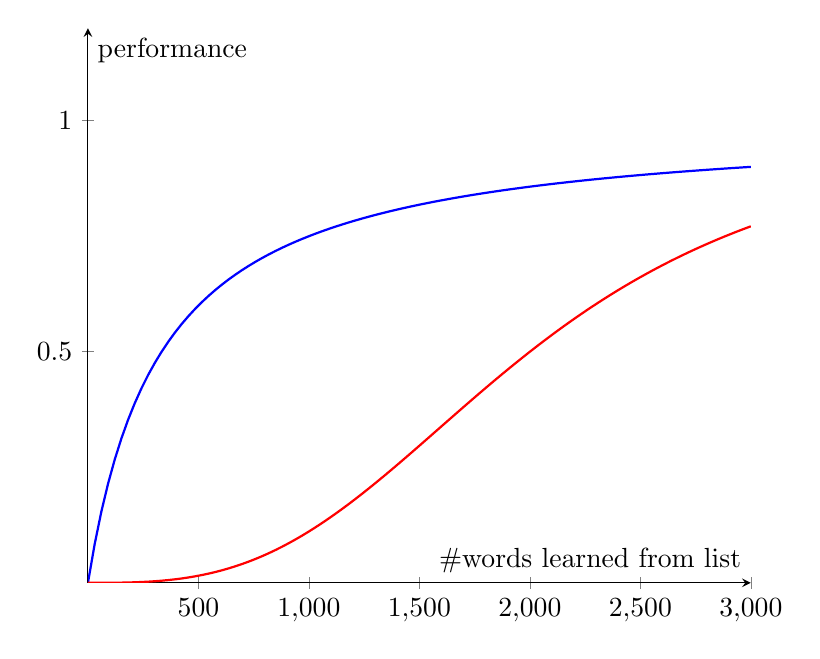
\begin{tikzpicture}
		\begin{axis}[
				axis lines = middle,
				xlabel = {\#words learned from list},
				ylabel = {performance},
				xtick = {0,500,1000,1500,2000,2500,3000},
				ytick = {-1,-0.5,0,0.5,1},
				samples = 100,
				domain = 0:3000,
				ymax=1.2,
				width=10cm
			]

			%curve
			\addplot[blue, thick] {1 - (1/((0.003*x)+1)};
			\addplot[red, thick] {1 - (1/(((0.0005*x)^3)+1)};
		\end{axis}
	\end{tikzpicture}
	\caption{Visualization of vocabulary list efficiency: \textbf{\textcolor{blue}{Blue}} represents the score with learning with an efficient list, \textbf{\textcolor{red}{Red}} represents the score learning from a less efficient list (i.e, less useful words at the top of the list)}
	\label{fig:voc-list-efficiency}
\end{figure}

\section{Experimental Setup: Measuring Word Utility as Ability Improvement in Humans} \label{sec:human-efficiency-testing}
With the formula \ref{eq:optimal-vocab-list}, we now have set our goal more concretely.
We are left with the question of how to design an actual experiment to test vocabulary list efficiency, and also how to generate one that is approximates an optimal list.
Hence, this section lays forth a hypothetical experiment design by using a human test subject to test efficiency, which will, however, be found to suffer from problems of feasibility, our solution to which is explained in Section \ref{sec:experimental-setup-with-ai}.

\subsection{Experimental Setup}
Let us first consider an example scenario, where we wish to measure the efficiency of one vocabulary list $l_A$ at $k=200$, $k=500$ and $k=2000$ words:
First, we would need to find a human test subject $s$ who does not know any words of the target language at the outset.
We then make the subject learn the words from $l_A$ one by one.
Once the subject seems to know 200 words, we perform a language exam and note their score.
Finally, we repeat the process for 500 and 2000 words.

\subsection{Problems of the Setup}
While this test setup might take a long time to complete for high $k$ values, it is still feasible.
But if we wish to compare the efficiency of $l_A$ with a second list $l_B$, we must measure how the same subject performs if they learn from the second vocabulary list, which presents is an unavoidable issue:
\textbf{The test subject cannot arbitrarily forget the words they have learned from the first list $l_A$.}
The experiment is thus not repeatable.

If we tweak the experiment such that each vocabulary list is learned by a different test subject, we introduce differences in capabilities between test subjects, making the evaluation of the list's efficiencies much more complicated to measure.
To make up for these inconsistencies, we might boost the number of test subjects to the point where each list is learned by a statistically significant group of subjects, but this would cause a sharp increase in the cost of the experiment.

However, this theoretical test setup could be feasible using a non-human test subject:
Using AI models and Explainable AI to analyze their interaction with language, we could not only evaluate, but even compile lists with drastically reduced costs.
This approach is laid out in the following sections.

\section{Experimental Setup with AI Model} \label{sec:experimental-setup-with-ai}
This work is interested in finding vocabulary lists that language learners can use to gain linguistic competence in their chosen field in the least possible time.
Section \ref{sec:formal-problem-statement} has specified how with the help of a proxy task, we can define this efficiency.
Section \ref{sec:human-efficiency-testing} has suggested a hypothetical experiment for testing the efficiency of a vocabulary list with human test subject.
However, we have established that the experiment is not easy to set up consistently, as it cannot be repeated with the same test subject on different lists, and a large pool of test subjects either means lower comparability of the scores or significantly increased costs.

To circumvent this issue, this work proposes the following idea:
To replace the human test subject in the experiment described in Section \ref{sec:human-efficiency-testing} with an AI model, facilitating a consistent and economical setup.
The following paragraphs discuss how, in such a setup, we can model the concepts from Section \ref{sec:statement-of-goal} such as linguistic context and utility with technological tools.

\subsection{AI as a Test Subject} \label{sec:ai-as-test-subject}
In recent years, AI models such as BERT have become highly adept at language-related tasks such as masked language modeling, question answering  and sentiment detection \cite{kentonBertPretrainingDeep2019}.
Such models possess an "understanding" of language that extends to the meaning of words:
They can recognize that two words such as "building" and "apartment" are close to each other in meaning, even though the words are dissimilar on a character level (this work makes no claims as to whether this ability stems from conscious understanding in the sense of the Chinese Room thought experiment \cite{searleMindsBrainsPrograms1980}, only that the models behaves as though they possessed such an understanding).
Thanks to this semantic language "understanding", AI models surpass the purely statistical approaches that were the paradigm of NLP until recently \cite{jurafskySpeechLanguageProcessing2025a}.
Thus, instead of a human who performs a language exam as described above to analyze their increases in linguistic understanding, we could let an AI model perform an NLP task on a corpus instead.

If we run the model on a specific corpus and mask some of the words in the input, it is expected that the performance will decrease in comparison to the full input.
However, presumably some words will have a larger impact on the performance than others.
If we view removing words from the input as the equivalent of a human not knowing a word in a text, this performance differential can be a proxy metric for word utility and for human language ability.

\subsection{Modified Experimental Setup with AI} \label{sec:ai-experiment-setup}
With this new proxy metric for word utility in mind, we can propose a new experiment.
To test the efficiency of a vocabulary list, we modify the setup from \ref{sec:human-efficiency-testing} as follows:

Let a pre-trained AI model perform its NLP task on a corpus.
At the start, we mask all the tokens in the input to simulate a language learner who is a complete beginner and thus knows no words in their target language.
We then progressively unmask the words from the vocabulary list in the input, and each time run the AI on the corpus to check the updated (and presumably improved) performance.

This yields a plot of performance over the number of unmasked words which shows how quickly the performance improves with unmasked words, similar to Figure \ref{fig:voc-list-efficiency}.
A quickly increasing performance corresponds to an efficient vocabulary list, whereas an inefficient list creates a plot with low initial gains in performance.

The modified experiment addresses the two issues proposed with the original setup:
It is cheap when compared to using a human test subject and unlike the human, the AI model has no memory of previous tests, meaning we can run the experiment consistently every time.
Next, let us see how the components in this setup interact with each other to model the concepts introduces in Section \ref{sec:statement-of-goal}:

\subsection{Influence of the Components on the Result}
The evaluation of the vocabulary list efficiency in the experiment will depend on the following components:

\begin{itemize}
	\item The AI model employed
	\item The input corpus
	\item The NLP task used
\end{itemize}

We have already addressed the role of the AI model in Section \ref{sec:ai-as-test-subject}.
The corpus and the NLP task performed by the model will also influence how quickly the AI model's performance increases with a given vocabulary list:

For example, when performing sentiment detection, words relating to emotion such as "hate", "like", "amazing" will matter more than for an Information Retrieval task such as Temporal Tagging.
The corpus has a more obvious influence on the performance, since corpora differ in many aspects such as formality, topic, and format of the text, all of which are components of a linguistic context.
Thus, by using diverse corpora, we can model various language contexts, and test word utility in those contexts.
Once we have efficient vocabulary lists across those contexts, a language learners could choose one or several of these lists, based on what linguistic context is closest to their language learning goals.

Table \ref{table:concept-implementation-correspondence} summarizes the correspondences between the concept and the technical component.

\begin{table}[ht]
	\centering
	\begin{tabularx}{\textwidth}{|X|X|}
		\hline
		\textbf{Abstract concept} & \textbf{Technical Implementation}  \\
		\hline
		Test subject              & AI model                           \\
		\hline
		Language ability          & Performance in NLP task            \\
		\hline
		Language context          & Corpus                             \\
		\hline
		Word utility              & Impact of word on task performance \\
		\hline
	\end{tabularx}
	\caption{Correspondence of abstract concepts to parts of implementation.}
	\label{table:concept-implementation-correspondence}
\end{table}

The next section discusses how we can not only test list efficiency, but make lists that approach an optimally efficient list.

\section{Evaluating vs. Making Lists of Useful Vocabulary} \label{sec:eval-vs-creation}
The previous section describes an approach for evaluating the efficiency of vocabulary lists, which measures how quickly the list lets a learner improve their understanding in a specific context.
While it can be seen as an improvement on the human setup because of its improved consistency and economy, it describes only the process of evaluation, not generation.
Actually finding optimal vocabulary lists is theoretically possible by testing every possible vocabulary list with all words in the language.
In practice, however, this would require an enormous amount of computational resources, as can be seen on a simple example:

Let us suppose we wish to find the most efficient vocabulary list of 1,000 words for some context.
To speed up list generation, we can make a preselection by allowing only the most frequent 20,000 words in the context as candidate members of this list.
This would yield a total number of $P(20000, 1000) = \frac{20000!}{19000!}$ possible vocabulary lists, all of which would need to be tested for efficiency to find the most efficient one.

We can optimize the evaluation process, however, since these tests consist of running the proxy task with a gradually increasing vocabulary, and each vocabulary is used in the evaluation for many vocabulary lists.
For our example, a vocabulary is a set of words formed by taking the first $n$ elements of the vocabulary list where $n \in [0, 1000]$.
If we only consider the number of possible vocabularies with a cardinality between 0 and 1,000, we get
$
	\sum_{k=0}^{1000} \binom{20000}{k} \approx \frac{1}{2} \times 2^{20000} = 2^{19999}
$ runs of the proxy task. Clearly, this is still an unfeasible amount of computation.

It can thus be seen that finding optimal vocabulary list is much too expensive when performed with a brute-force approach.
For this reason, the next section introduces an alternative method for finding efficient lists of vocabulary, based on XAI as a tool which extracts information about the linguistic skills of AI models.

\section{Generating Efficient Lists of Vocabulary} \label{sec:list-generation}

The previous sections have shown the challenges in evaluating the efficiency of vocabulary lists with human test subjects, and suggested a repeatable approach utilizing AI models, NLP tasks and corpora to overcome these challenges.
We have seen, however, that this approach does not suffice to generate efficient vocabulary.
Therefore, to achieve cost-efficient list generation, this section advocates for adding a final component to our experimental setup, namely Explainable AI.

\subsection{Explainable AI as a Tool of Analysis} \label{sec:xai-as-tools-of-analysis}
The guiding question of this thesis is:
\textit{Which words provide the most language understanding in a given linguistic context?}.
Section \ref{sec:experimental-setup-with-ai} has put forward an experimental setup in which the concepts of language understanding and context are simulated with technological components.
By substituting these terms, the question is turned into:
\textit{Which words provide the highest improvements in performance of an AI model performing an NLP task on a given corpus?}.

Put like this, the question is very close to the questions that the field of Explainable AI seeks to answer.
A typical question of Explainable AI would be:
\textit{Why, for a given input, does the model arrive at its output?}. 
To be more precise, this is a question for a \textit{local} explanation (see Section \ref{sec:xai-methods}).
As mentioned in Section \ref{sec:xai-methods}, we use feature importance attribution methods, which, for an NLP task, transforms the question into:
\textit{Which words in the input have the most influence on the model arriving at its output?}

By answering this question on a statistically relevant sample of individual inputs from a corpus, we can find out which words are the most essential for the AI model to perform its task in the corpus overall.
If the words found in this way are close to those that would provide the most utility to a human learner as well, they could be used to create very efficient vocabulary lists as well.

Once we have calculated the utilities of words, we only need to sort the words by their utility to arrive at a vocabulary list that should be close to optimally efficient.
It must be noted that this is only an approximation of a maximally efficient list.
This is because, theoretically, the utility of two words combined could be higher than the sum of their individual utilities.
In other words, our approach ignores possible synergistic effects between words.

By adding XAI as a tool for analyzing the interaction of the AI model with the corpus, we finally have an experimental setup for generating efficient vocabulary lists.
This is not a replacement of the approach described in Section \ref{sec:experimental-setup-with-ai}.
Rather, this work uses the generation approach to make lists (Chapter \ref{ch:implementation}), and the evaluation approach for testing which of these lists are the most efficient (Chapter \ref{ch:evaluation}).
In the next section, we discuss the implementation of this approach.
We present various choices for these components, and argue for some to be used over others, with the aim of making the utility estimated by the framework align as much as possible with utility to human learners.


\chapter{Implementation} \label{ch:implementation}
Chapter \ref{ch:approach} has formalized the problem and put forward a novel framework for finding useful words, consisting of two major functionalities:
Vocabulary list generation, and vocabulary list evaluation.
The list evaluation approach, described in Section \ref{sec:experimental-setup-with-ai}, utilizes the performance of an AI model, corpus, proxy task as a proxy metric for language ability, in order to estimate how efficiently the vocabulary list may help a human language learner acquire competency.
The list generation approach, proposed in Section \ref{sec:list-generation}, additionally uses Explainable AI as a tool for analyzing the interaction of the AI model with the corpus to compile vocabulary lists that approach maximal efficiency.

In this chapter, we will describe our implementation, mostly of the list generation approach.
This is because the list evaluation method will be used in Chapter \ref{ch:evaluation} as one among several metrics for evaluating the efficiency of vocabulary lists generated by the implementation in this chapter.
However, the evaluation with our approach will use the same components as the list generation approach, such as the chosen corpora, AI models, and NLP tasks.

The first section describes the implementation of the list generation approach from a system design perspective, describing the interaction between the individual components.

The choice of components in the system is then argued in the following sections, each of which will feature section describing the desiderata of the component choice are and why, followed by the selection of concrete components.
\todo{Write rest of introduction when chapter structure stands. }

\section{Data Pipeline}

This section will give a top-level overview of our implementation for the list generation approach described in Chapter \ref{ch:evaluation}.
As mentioned before, the main components of this approach are:

\begin{itemize}
	\item An NLP task, which models a language ability of a language learner.
	\item An AI model, used as a test subject.
	\item A context-specific corpus, to model a language context.
	\item An XAI method, which analyzes the interaction of the AI model with the corpus to determine word utilities.
	\item If the XAI method allows: A tokenizer, determining the words to be analyzed.
\end{itemize}

Thus, the implementation of the approach will consist of determining how exactly these components interact, as well as deciding which model, which XAI method, etc., will be used.
The interaction of these components can be seen in pseudocode in Algorithm \ref{alg:efficient-list-generation}.

\begin{algorithm}
\caption{Efficient List Generation.}
\label{alg:efficient-list-generation}
\begin{algorithmic}[1]
\Require corpus, model, xai\_method
\State Initialize $line\_word\_utilities\_scores$ with empty list

\For{each $line$ in $corpus$}
    \State $word\_utilities\_for\_this\_line \gets$ xai\_method$(model, line)$
    \State Append $word\_utilities\_for\_this\_line$ to $line\_word\_utilities\_scores$
\EndFor

\State $corpus\_word\_utilities\_scores \gets$ aggregate\_word\_utilities($line\_word\_utilities\_scores$)

\State $voc\_list \gets$ words ordered by $corpus\_word\_utilities\_scores$

\State \Return $voc\_list$
\end{algorithmic}
\end{algorithm}


The choice of individual components will be tackled by the following sections.
Because of some dependencies between the components, not all of these components have their own sections
The NLP task performed depends on the AI model that we use, as most AI models are trained on only one task.
Therefore, the choice of AI model is discussed together with the NLP task in the next section.

\section{NLP Tasks and AI Models}
The NLP task and the corpus used for list generation

There are many NLP tasks we could choose from \tocite{huggingface NLP task list or something}.
But not all are equally suitable.
This section will first put forward criteria for selecting NLP tasks in Section \ref{sec:nlp-tasks-desiderata} for word utility evaluation.
% After this, we use these criteria to select a few NLP tasks as appropriate in Section \ref{sec:nlp-tasks-selection}.
After the final selection, we will be left with two tasks which, in the estimation of the author of this work, are the most suitable for our word utility evaluation approach, namely \textit{Next Sentence Prediction} and \textit{Sentence Embedding}.
These NLP tasks we choose dictate the format of our input data, i.e., the corpora we can use.
Therefore, the selection of corpora will be discussed after the choice of NLP is finalized.

\subsection{Desiderata} \label{sec:nlp-tasks-desiderata}

\contentdescription{
	{
			\begin{itemize}
				\item Support many languages
				\item Be as close to human need as possible
				\item $\rightarrow$ task should show general language understanding
				\item data is easy to acquire
				\item $\rightarrow$ data should be freely available for lots of contexts
				\item $\rightarrow$ no need for manual labeling of data
			\end{itemize}
		}}

This section will put forward four criteria for selecting NLP tasks for word utility extraction:
The availability of many multilingual AI models and corpora usable as input for the task, generality of the task and ease of evaluation.
These criteria will be used in the next section to select concrete tasks for our implementation.

\subsubsection{Model Availability in Many Languages}
The goal of this work is to find approaches to find useful words for the purpose of language learning.
Much research in Natural Language Processing is dedicated to improving NLP performance in English and other high-resource languages such as Spanish, French or Mandarin Chinese \tocite{resource availability in various languages}.
This has the consequence that many AI models and other NLP methods achieve high levels of performance only in these languages, and many AI models are only available in English or only a small number of languages.
However, there are over 7,000 languages in the world \tocite{Ethnologue}, and for many of these there exist corpora, or online digital texts which could hypothetically be used as inputs for our word utility extraction approach.
For this reason, our implementation strives to realize word utility extraction in \textbf{as many languages as possible}.

\subsubsection{Corpus Availability in Many Languages}
The second point of consideration for task selection is \textbf{how much data is available for performing the task}.
Ideally, we would like tasks for which suitable corpora are freely available or can be trivially generated from available corpora.
This is for the reason that, with a larger amount of usable data, we not only improve the accuracy of our approach, but also increase the diversity of input data.
With diverse input data available, we have a larger amount of linguistic contexts for we can find utilities, and the context-specific language learning is a central motivation of this work.

\subsubsection{Generality of Skill Required}
Another important point to consider when selecting an NLP task is \textbf{how general the linguistic skills} are that the task requires:
We use the performance in the NLP task as a proxy metric for the test subject's language ability.
As such, we must ensure that task reflects a general level of semantic understanding, not only a narrow mechanistic skill that can be accomplished by using only a small part of the input.

\subsubsection{Ease of Evaluation}
To ensure we can measure the performance, we must also choose a task whose results can be easily compared with each other:
Some tasks, such as text summarization, present a challenge for automatic evaluation:
It is difficult to put a number on how similar two summaries of a text are.
While evaluation measures, such as BLUE scores\tocite{BLEU}, exist, it is questionable how well they capture the similarity between texts, because they do not recognize the semantic similarity of synonyms, and a different sentence structure will result in a low BLEU score even if the actual meaning of the sentences may be very close.
It follows that if we have the freedom to choose NLP tasks whose results can be automatically evaluated with a fair degree of accuracy, we should choose them.


\subsubsection{Summary}
To summarize our desiderata for NLP tasks:
Our implementation seeks to use NLP tasks for which both AI models and corpora exist in a large number of languages, to maximize accuracy and diversity of linguistic contexts which can be modeled.
We prefer tasks that demonstrate general language understanding over tasks that only require a narrow skill set to perform or that are too technical, because general tasks are expected to align more with human linguistic skills.
Finally, the task must be easily scorable, since the task score is the metric by which we gauge how useful words are.

The next section will present several tasks which fulfill the above criteria, and explain what consequences their selection has on the other components of vocabulary list generation.
The choice of NLP tasks employed to test a XAI-based approach for word utility estimation is a crucial step:
Since we are trying to estimate utility by measuring the impact of a word on language understanding, the NLP tasks should reflect language understanding as much as possible.

\subsection{Survey of Candidate NLP Tasks}
This chapter introduces some NLP tasks that might work for our purposes.
We will describe first the process of how candidate tasks were found, and then go into detail for each candidate as to why it was or was not selected in the following subsections.

Candidates were first compiled by surveying common pre-training tasks which are of state-of-the-art NLP models:
This is because the purpose of a pre-training task is to endow the AI model with a general understanding of the language, before either using transfer learning to specialize it for a more specific downstream task, or using it before another downstream AI model to pre-process input \missingcitation{definition of pre-training task}.
Such tasks must necessarily be general and require general language understanding, since training the model with them is supposed to provide a solid basis for a wide variety of NLP tasks.
Another benefit of using pre-training tasks is that their training is unsupervised, meaning there is no need to manually label data.
Their widespread use in \NLP also means that pre-trained models are widely and freely available.

\subsubsection{NLP Pre-Training Tasks Used by State-of-the-Art AI Models}
This section takes a look at the pre-training process of recent state-of-the-art LLM models which have made public their training process.
Both the NLP tasks and the kind of data is considered.


\begin{description}
	\item[GPT-4] \cite{openaiGPT4TechnicalReport2024}

	      Task: Language modeling (see next section).

	      Data: Not disclosed in detail, according to the original paper, the model was trained "using both publicly available data (such as internet data) and data licensed from third-party providers".
	\item[GPT-3] \cite{brownLanguageModelsAre2020}
	      GPT-3 is a model that does not rely on transfer learning to apply its linguistic understanding to new tasks; instead, it uses zero-shot and few-shot learning to perform tasks it was not specifically trained for.

	      Task: Language modeling (same as GPT-2 \cite{radfordLanguageModelsAre2019})

	      Data: Common Crawl, WebText2, Books1, Books2, Wikipedia \todo{link sources?}
	\item[LLama 3.3] \cite{LlamamodelsModelsLlama3_3}


	      Task: Meta did not make public the training process for Llama 3.3.

	      Data: "data from publicly available sources"
\end{description}

\subsubsection{List of Candidates}
\begin{description}
	\item[Next Sentence Prediction]
	      In this task, the AI model takes as input two sentences and predicts a probability for the second sentence being the successor of the first sentence in their source text.
	      Advantages for this task for our purposes is that such a dataset is easy to generate, as it merely requires a corpus of sentences that follow from each other, which is easily obtained from Wikipedia articles, film subtitles, or any other continuous text.

	\item[Text summarization]
	      This task involves summarizing a given text, in other words, writing a shorter version of the input text while still conveying as much of the information from the original text as possible.
	      Summarizing texts seems to require a high level of "understanding" of the text and would thus seem to be good choice for testing whether ablating certain words from the text would have detrimental effect on the model performance.
	      Unfortunately, this task requires hand-labeled datasets and is thus not a good candidate if we aim to find approaches which can be implemented in many different languages, as there is a dearth in data in many of the less-studied languages of the world.

	\item[Masked language Modeling (aka. "cloze task")]
	\item[Causal Language Modeling (aka. Next token prediction)]
	\item[Sentence order prediction]
	\item[Sentence embeddings]
	      Sentence embeddings take the approach of transforming words into meaningful vectors and extend it to whole sentences.
	      This "task" differs from the others in that we do not measure differences in performance when the input is perturbed; but rather a distance between the embedding vectors themselves.
	      This justification for such an approach is that sentences whose meaning is very different should end up further apart from each other in the vector space once embedded.
	      This brings several advantages:
	      This approach can be performed on any corpus containing distinct sentences.
	      These corpus does not have to be document-level, and sentences need not be consecutive.
	      To make this a task on which XAI methods can be applied, we can define a distance from the original token
\end{description}


\section{Next Sentence Prediction}

\begin{description}
	\item[LASER] \cite{artetxeMassivelyMultilingualSentence2019}
	\item[BERT] \cite{reimersMakingMonolingualSentence2020}
\end{description}

\subsection{Choice of Model}
\subsection{Data Required}

Requires a corpus that contains consecutive sentences.
Furthermore, NSP typically predicts whether two sentences follow each other in a document, not a dialogue (see the data on BERT training \cite{kentonBertPretrainingDeep2019}).
This excludes movie subtitles from the possible corpora for this task.


\section{Sentence Embedding}
\subsection{Choice of Model}
\subsection{Data Required}


\todo{tests of performance tests of models used with corpora used (e.g., if NSP prediction model is reliable)}


\section{Corpora}
The previous section has put forth criteria for which NLP tasks should be used in our word utility evaluation approach.
The other core component of the approach is the input data used to perform the experiments, as it serves the purpose of modeling the language contexts in which the language learner is striving to achieve proficiency.
This section will therefore first lay out the general selection criteria for corpora.
We will then introduce some publicly available corpora which are suitable for our evaluation approach, as well as propose data augmentation methods to increase their usefulness further.



\subsection{Desiderata}

\contentdescription{
	{
			For the purposes of this work, it was desirable that the corpora used be:
			\begin{itemize}
				\item representative of what language learners strive for
				\item freely available in many languages
				\item can be split up into diverse linguistic contexts
				\item for NSP: must be comprised of documents for continuous sentences
			\end{itemize}
		}}

This section will put forward our general criteria for corpus selection, following from our overarching goal of using the model to model linguistic contexts for the purpose of language learning.
\todo{when the following subsection stand, summarize here}
\todo{when actual corpora are decided: Mention them in throughout this section too}


\subsubsection{Document-Level Corpus}
The first desideratum for our corpora stems from our choice to use Next Sentence Prediction as one of our NLP tasks:
As Next Sentence Prediction predicts whether one sentence is likely the continuation of another, it requires continuous sentences pairs to work.
To generate these pairs, we must use (at least some) corpora featuring continuous tests, not only individual sentences.
This presents a challenge, as many corpora which are compiled from Web Crawls, such as the Common Crawl dataset \footnote{\url{https://commoncrawl.org/}}, present independent single lines, mostly because single sentences cannot be put under copyright in many states \tocite{copyright being the reason for non-document level corpora}
One solution to this would be make a dataset from crawling various news pages ourselves.
However, Wikipedia contains articles on many different topics which do not underlie strict copyright license (see the section on Wikipedia), thus for this work, we opted not to compile our own document-level corpus.

\subsubsection{Free Availability in Many Languages}
In Section \ref{sec:nlp-tasks-desiderata} we put forward reasons for why freely available AI models which can handle a diverse pool of languages are desirable for our undertaking.
By the same token, we also prefer corpora which are publicly available in many languages over corpora which only include data in one language.
While a monolingual corpus is not inferior to a multilingual one, its use necessitates that the user manually compile many corpora if a multilingual implementation is to be achieved.

\subsubsection{Closeness to Linguistic Contexts Desired by Language Learners}
As mentioned before, the corpus in our word utility extraction approach serves the purpose of modeling a linguistic context, and this linguistic context should reflect some set of situations that a language learner is likely to find themselves in.
Typical situations would include reading the news, reading literature or watching movies in their target language.
As such, corpora which are close to the materials which language learners are likely to engage with are desirable, since their use makes the AI model's performance on the task more reflective of skills that a language learner would like to acquire.

\subsubsection{Diversity of Linguistic Contexts within Corpus}
Not only the relevance of the entire corpus's linguistic context is important:
Some corpora enable us to further split them up into smaller corpora with more specific language contexts.
For instance, while we can use a corpus such as \textit{Wikipedia} as a whole, the structure of Wikipedia enables us to group articles by the category they belong to (politics/sports etc.), as well as split them by subheading (History/Introduction/etc.) to find more specific contexts.
Such corpora are especially efficient for generating multiple contexts, hence we will make use of such corpora.



\subsection{Corpora Used}

\subsubsection{Background Corpus: mOscar}
For the implementation of TF-IDF, we require a generic background corpus to normalize raw word frequencies found in context-specific corpora (that is, to calculate the IDF part of TF-IDF).
For this purpose, corpora crawled from the internet offer themselves as a diverse option:
While we cannot be certain if some kinds of web pages will feature disproportionately in the final corpus, web content is diverse in that it encompassed both formal and informal content on many different topics.

A natural choice of diverse web content is the \textit{Common Crawl} dataset \footnote{\url{https://commoncrawl.org/}}.
However, in its raw form, it takes the form of HTML code and includes much boilerplate content such as cookie requests, necessitating much preprocessing.
Another major downsize of \textit{Common Crawl} is that its data is not categorized by language, meaning we would have to perform language categorization as an additional preprocessing step before using it for our purposes.
We also rejected the \textit{Wortschatz Leipzig} Web Corpora because, while these corpora are stripped of any HTML code, they are lines taken randomly from websites, rather than whole documents.
The original paper for the \textit{Wortschatz} corpus also mentions political content was utilized to bootstrap in the web searches for data gathering, including the \textit{Universal Declaration of Human Rights} and the Jehova's Witnesses magazine \textit{Watchtower} \footnote{Previously available at \url{watchtower.org}}, which may lead to a respective bias in the final corpus.

Finally, a corpus from the \textit{Oscar} project \footnote{\url{https://oscar-project.github.io/}} was chosen as a background corpus:
Each \textit{Oscar} corpus is a cleaned-up version of a \textit{Common Crawl} dataset, on which preprocessing steps such as HTML stripping and removal of boilerplate content have already been performed.
It consists of (whole) web pages, and most importantly, its content is language-tagged, covering more than 150 languages in total.
There exist many versions of the Oscar dataset, but this work, the \textit{mOscar} \cite{futeralMOSCARLargescaleMultilingual2024} corpus from 2024 was chosen, both for its recency and coverage of many languages.

\todo{State number of documents used from Oscar corpus}

\subsubsection{OpenSubtitles Parallel Corpus}
This set of corpora contains parallel corpora:
Corpora which has text segments in one language aligned with the presumed translation of the segment in a second language.
Its sentences are generated from subtitles from the popular subtitle sharing platform \textit{OpenSubtitles} (https://www.opensubtitles.org/) and undergo various preprocessing and filtering steps as described in \cite{lisonOpensubtitles2016ExtractingLarge2016}.
These include:
\begin{enumerate}
	\item Enforcing universal UTF-8 character encoding.
	\item
	      Splitting and joining of sentences from their original subtitles blocks (the segments which appear on-screen when watching the movie with its subtitle).
	      One such block may contain multiple sentences, or only a partial one.
	      There is thus an n-to-m-relationship between the blocks and sentences.
	\item Checking and correcting possible spelling issues, especially ones arising from OCR (Optical character recognition) errors.
	\item From available subtitles, identifying the subtitle pair which is most likely to be accurate in its alignments and free from errors such spelling, taking into account metadata such as user ratings of subtitles.

\end{enumerate}
One advantageous aspect of this corpus is that it contains many sentences that are sequential, which means we can generate a Next Sentence Prediction dataset from it (add hedging here since not all lines in corpus are sequential and even within the same movies there may will be pauses in the subs).
This corpus has been used to train machine translation models such as OPUS-MT \cite{tiedemannOPUSMTbuildingOpenTranslation2020}, a freely available set of transformer models for translation, including between low-resource languages. \todo{Not completely correct, the pipeline uses data from OPUS, not necessarily or specifically from OpenSubs}
While it is possible to reconstruct which movies the subtitle lines came from information contained in the corpus, it is unfortunately not clear how these movies were selected in the first place.

The full process, as illustrated by the authors, can be seen in Figure \ref{fig:opensubs pipeline}
As of 2025, the latest version of the corpus (v2018) contains aligned subtitles of 62 languages between each other.

\begin{figure}[H]
	\centering
	\includegraphics[width=\textwidth]{opensubs_corpus_processing.png}
	\caption{The pipeline producing the OpenSubtitles parallel corpus}
	\label{fig:opensubs pipeline}
\end{figure}

\subsubsection{Wikipedia}
\contentdescription{{
			\begin{itemize}
				\item advantages: diversity of topics, document level corpus which is not copyrighted, regularly updates dumps
				\item disadvantages: language is technical, does not resemble spoken conversation
				\item describe grouping intro multiple scope corpora: describe category structure of Wikipedia
			\end{itemize}
		}}

Wikipedia offers a large amount of data which can be downloaded in the form of dumps at \url{https://dumps.wikimedia.org/}.
In this work, these dumps will be valuable in modeling various linguistic contexts that a language learner might be interested in.

\paragraph{Advantages:}

Wikipedia is a valuable resource for several reasons:
It contains a vast number of articles, from a diverse set of topics.
Wikipedia articles have categories assigned to them, which we can use to group articles into linguistic contexts.
This means we do not have to assign the articles to topics ourselves, thus enabling the creation of many smaller-scope corpora from Wikipedia with minimal effort.
The characteristics of the article category system on Wikipedia will be discussed in the paragraph below.

Another upshot of Wikipedia is that its articles are licensed under the Creative Commons Attribution-ShareAlike 4.0 International License (\textit{CC BY-SA}).
Because of this, Wikipedia can provide dumps of its entire article database ready for download, with the articles in continuous form and with category metadata attached to them.
This enables us to use the articles as a source for Next Sentence Prediction NSP task.

\paragraph{Disadvantages:}
While Wikipedia offers a large diversity of articles and article topics, the language of the articles follows an academic style of writing.
Thus, the diversity in registers is comparatively low:
Wikipedia is less likely to contain informal language, such as nonstandard language (English: \textit{ain't}, \textit{y'all}) and slang.

Furthermore, it features little language taking conversational form.
% This means that e.g., for English, the second person pronoun "you" occurs very infrequently on Wikipedia. \tocite{Wikipedia rank of you}
This is especially relevant for languages where the certain grammatical forms signify something about the relationship between the speaker and listener:
In Japanese, there exist various linguistic markers of politeness (\textit{Teineigo} and \textit{Keigo}) which play a crucial role in in-person interactions between Japanese speakers, as their presence or absence can signify respect, familiarity or humility with regard to one's interlocutor.
However, such forms are rarely found on Wikipedia, as it does not take the form of a person addressing another person or persons.
Thus, we can see that texts on Wikipedia are of limited use to model linguistic contexts involving in-person conversion.

With these advantages and disadvantages in mind, this work uses Wikipedia articles and their associated metadata to make corpora of various sizes, as will be seen in the next section.

\paragraph{Modeling Linguistic Contexts}

One of the chief advantages of Wikipedia as a corpus its diversity of covered topics.
A language learner who is interested in a particular topic will likely find a matching article category on Wikipedia:
For example, a person with an interest in American cinema who is learning English could likely take vocabulary from the articles of the category "20th-century American actresses" to boost their language learning in that linguistic context.
For this reason, we use a number of manually selected categories as testing grounds for our list generation approach.
For each category, we use a number of articles to make a list, then use different articles from the same category as testing data in the evaluation.
We can thus check if learning vocabulary from a category genuinely prepares a learner in understanding texts from that context.

At the same time, a learner could also wish to make a vocabulary list from concrete Wikipedia articles they would like to read.
For that reason, also use single articles as corpora to be processed by our list generation approach.
In that case, no split of training and test data is necessary, as the aim is not to model general knowledge about a domain, but equip the learner with vocabulary about the \textbf{closed} context of a Wikipedia article.
Therefore, in the single-article approach, both the list generation and evaluation use all lines of the article.


% \paragraph{Wikipedia's Category System for Articles}
% There are x categoris on Wikipedia.
% Each article may belong to one or more categories.
% One category can have 0:n parent categories, 0:n child categories.
% Categories therefore not not follow a tree structure, thus most articles belong to more than one top-level category.



\subsubsection{Leipzig Wortschatz Corpora}
Available in x languages

But: data quality issues, methodology might be outdated

\cite{goldhahnBuildingLargeMonolingual2012}

\subsubsection{CCMatrix / NLLB}

% \subsection{Data Augmentation}
% Data Augmentation was not used to gain additional data.
% While in recent years data augmentation methods have become popular for training AI models in NLP, most of these would have either no or a detrimental effect on the methods employed in this work
% Some of these methods include \cite{pellicerDataAugmentationTechniques2023}:
% \begin{description}
% 	\item[Character level]
% 	      Introducing character swaps to data is a method used to train the model to noise in the data, but in our case, would only add noise to the results.
% 	\item[Word level]
% 	      There exist techniques to switch words for synonyms or swap words in the sentences to create noise.
% 	      As with noise on the word level, adding words in inappropriate places is undesired for our use case.
% 	      Swapping words for synonyms would also prove detrimental, as this would skew the statistics away from the natural word distribution found in the human-generated source texts.
% \end{description}
% Higher level techniques suffer from the same issues.
% For this reason, the data is left in its "natural state" for our purposes.
%

\section{XAI Methods} \label{sec:xai-methods}
In order to appraise the influence of words in a corpus on the performance of the AI model performing and NLP task, this work employs Explainable AI methods, as explained in Section \ref{sec:xai-as-tools-of-analysis}.

\subsection{Desiderata}
Section \ref{sec:explainable-ai} has explained the use of XAI and stated what kind of XAI methods are especially appropriate for our purpose:
We will employ local, feature attribution XAI methods of both model-specific and model-agnostic type, as these will allow use to gauge the importance of words in the input from multiple points of view.
Model-specific methods have an advantage in that they typically do not require many model calls to attribute importances to features, and take the model structure into account.
On the other hand, model-agnostic methods are useful in that they can be used on any model and gauge the input-output relationship by performing actual experiments on the model, by observing the way changes to input change the output of the model.

In addition to these taxonomical specifications, an ideal XAI method for word extraction should be both accurate in its feature attributions and should not require extensive computation.
Apart from the benefit of attaining faster results, a computationally lightweight approach allows the model to process more data in less time, presumably boosting the accuracy of the resulting utility evaluation.

In the following sections, we will propose several concrete XAI methods for use with the described list generation approach.
The relationship of the XAI methods to the NLP tasks will also be discussed, as not every XAI method is feasible with every task, either because of unrealistic amount of computation or because the results of the combination are difficult to evaluate.
The results of the experiments with these methods will be seen in Chapter \ref{ch:evaluation}.
\todo{argue against approaches where the input is reduced to BOW, such as SHAP}

\subsection{Model-Agnostic Approaches}
\contentdescription{
	Single Token Ablation, Progressive Summary with
}

\subsubsection{Single Token Ablation}
Our aim in using XAI methods is to find out which words, if known, improve the model's performance the most, when compared to not knowing the word.
Perhaps the simplest way of testing this is by going through every word in the input to the AI model, and checking the model performance when the word is removed from the input.
Within this work, this approach will be known as \textbf{Single Token Ablation}.

\paragraph{Approach:}
Given an input line or a pair of lines:
For each word in the input, create a variation of the input where the word is removed.
Run the model on all inputs and measure how much performance is degraded in each case.
Estimated utility is the difference in performance between not removing and removing the word.

\paragraph{Advantages:}
One advantage of Single Token Ablation is its conceptual simplicity, as it is very easy to implement.
Furthermore, its time complexity is fairly minimal for a feature method, as it requires only one model call for each unique token in the sentence ($\mathcal{O}(n)$).

\paragraph{Disadvantages:}
The main downside of this method is that, in long sentences, leaving out a single token will not change the meaning of the sentence to such an extent that the sentence becomes unintelligible.
Assuming the AI model can process sentences with missing words with similar accuracy as humans, the impact on performance may therefore be minimal or not predictive of actual usefulness.
Furthermore, this method does not take into account the utility of a word in the context of word combinations.

\paragraph{Summary:}
Among model-agnostic methods, Single Token Ablation is a computationally inexpensive whose feature perturbation consists of ablating single words.
We may think of this method as simulating a language learner who already knows all words in a sentence except for one, and as such it may not model word utility in such a way that the resulting list is useful for beginners.

\subsubsection{Progressive Summary}
While Single Token Ablation is easy to implement and cheap to execute, its downside is that the performance differences may not be representative of actual utility.
To achieve a more accurate evaluation, we may think of an approach that is in some sense the inverse of removing single words from sentences:
Checking which words are the most essential by reducing the sentence a minimal number of words.

\paragraph{Approach:}
Given an input line, we first let the AI model run on the unaltered input.
We then go through every word in the input line, let the model run with the single word as input, and check which of the words produces an output that is close to the output for the unaltered line.
We can thus see which word summarized the sentence the best.

However, we need not stop here:
After determining the most essential word in the sentence, we can check which words from the remaining pool of words brings the outputs closer still.
By iterating this method, we progressively reconstruct the original sentence, which each step being the best next word to add in order to restore the original output.
For this reason, we will refer to this method as \textbf{Progressive Summary}.
Here, the estimated utility of a word is the boost in performance which is brought to the sentence when the word is added.

\paragraph{Advantages:}
The Progressive Summary approach models the perception of a beginner-level language learner better than Single Token Ablation.
The latter asks which single word, when lacking, degrades performance the most.
Progressive Summary instead asks which words, if known, bring language performance closest to knowing all words in the sentence.

\paragraph{Disadvantages:}
Progressive Summary is much more computationally intensive than Single Token Ablation, which requires only one model call per word in the sentence.
Because of its iterative approach, for a sentence with 10 words, Progressive Summary calls the model $10+9+8+... $ or $\sum_{i=1}^{n}i = \frac{n^2 + n}{2}$ times, which is a time complexity of $\mathcal{O}(n^2)$.


\paragraph{Compatibility with NLP tasks}
As Progressive Summary starts from a set of one words and then progresses to larger sets, it is difficulty to meaningfully employ in combination with an NLP task whose input is not a single line, e.g., Next Sentence Prediction.
One could circumvent the issue by leaving one of the sentences in its original form and only perturbing the other, but this can hardly be seen as a modeling of natural language ability.

\todo{Maybe: Describe issues of using PS with models whose output is single number: Approximating with single words may not be meaningful approximation at all. But should test empirically.}

As such, our implementation Progressive Summary is not used with Next Sentence Prediction.

\paragraph{Summary:}
Progressive Summary attempts to find the most important words in a sentence one by one, by first reducing the sentence to one word, then two etc., and using a distance metric to compare the "summaries" to the original sentence.
The words which bring the model output for the summary closest to that of the original sentence are regarded as the most useful.

\subsection{Model-Specific Methods}
The model-agnostic methods so far are general tools which can be employed on any model.
However, as many of the latest state-of-the-art AI models follow the Neural Network architecture, and more specifically the transformer architecture (see Section \ref{sec:transformer}), we will also attempt word utility estimation with methods specific to these model.
These model-specific XAI methods have the advantage of being computationally efficient:
Model-agnostic methods extract information about the model by perturbing its inputs and analyzing the resulting changes in the output.
This requires many model calls for one input datum.
In contrast, model-specific methods can analyze the input-output relationship with only one model call, as they look into the model itself for information.
We will therefore try two model-specific methods for analyzing word utility as well, as their more efficient calculations means they can process more input data in a given time, which should increase the accuracy of the resulting word list.

\subsubsection{Attention as Explanation}
One XAI method which has been proposed to explain the decision of transformer models specifically is the transformer's own attention mechanism:
As stated in Section \ref{sec:transformer}, transformer model (if their input is in text format) use self-attention to assign importance to the connections between tokens in the input.
This may be used as a kind of explanation, as words which have strong connections to many words in the sentences presumably are more important than those receiving less self-attention.

An important difference to the model-agnostic methods explained before is that we do not control word masking with a tokenizer \textit{independent of the model}, thus the splitting of words is not under our direct control.
The tokenizers used are \texttt{bert-base-uncased} and \texttt{sentence-transformers/paraphrase-MiniLM-L6-v2}.
These produce tokens on a sub-word level, which means that we must perform post-processing on the attentions to acquire values on the word level and make vocabulary lists than contain full words.
For BERT tokens, this is a simple process as sub-tokens which are not at the beginning of a word start with "\#\#".
\todo{Insert sub-word tokenization example from BERT}
The estimated utility for the reconstructed token is calculated by taking the sum of the attention values of each sub-token.

\paragraph{Approach:}
A transformer model is run with one line as input.
The transformer will output an attention tensor, which attributes a value to each pair of tokens in the input (this includes special tokens from the tokenizer, such as and \texttt{[SEP]} and punctuation).
We then aggregate the attention of each token by summing over one axis of the attention tensor of all connections each token has, and over all the attention heads, resulting in one scalar value per token.
The original tokens of the tokenizer are merged
Next, special tokens and punctuation are filtered
Finally, we normalize the attentions such that the attention for all words in the line sums up to one.
The attributed attention to a word is its estimated utility.

\paragraph{Advantages:}
As hinted at before, this method uses one model call for one input line, and thus has a time complexity of $\mathcal{O}(1)$.

\paragraph{Disadvantages:}
One disadvantage of Attention as our attention mechanism is that attentions are attributed to input tokens of the model.
Unlike the model-agnostic methods where word masking is controlled by a tokenizer \textit{independent of the model}, the tokenizer cannot be changed.
AI models are trained with some tokenizer as preprocessing the input, and this tokenizer cannot be changed, lest we change the input format to the AI model itself.
This is an issue because it means that lists generated with the model-specific tokenizer are not necessarily comparable to lists from model-agnostic methods, as the tokenization method may differ.

In addition to this technical downside, Attention is controversial as a mechanism to explain model decisions.
\tocite{Attention is not Explanation}

\paragraph{Summary:}
Among the XAI methods used in this work, Attention as Explanation requires the least resources, and it is not restricted to any one NLP task (although the model must be of transformer type).
However, we do not control the tokenizer used directly.
While the NSP model uses the same tokenizer that is also used for token masking in the model-agnostic XAI methods, the sentences embedding model uses a different tokenizer.



% \subsubsection{Layer-wise Relevance Propagation (not yet implemented $\rightarrow$ may be deleted)}
% \paragraph{Approach:}
% \paragraph{Advantages:}
% \paragraph{Disadvantages:}
% \paragraph{Summary:}
%
%

\chapter{Evaluation} \label{ch:evaluation}
\section{Selection of evaluation measures}

The various utility extraction approaches produce ranked lists as outputs.
To compare these, I employ both quantitative and qualitative comparison approaches, described in the following chapters.

\subsection{List similarities}
In order to compare the results provided by the various approaches, metrics are needed that can be consistently calculated across the different approaches.
While a human may be able to qualitatively analyze lists and gain a rough idea of their similarity, computed metrics provide an instantaneous (if simplified) outlook on similarities.
A metric shall be defined as a function which takes as parameters two word lists of equal length which are word lists ordered descendingly by supposed relevance, and outputs a real number giving either a distance or similarity between the lists.

Considerations of the choice of metric are:

\begin{description}
	\item [Handling of lists with partial overlap.]
	      Metrics must be able to handle elements which occur in only one of the two lists.
	      Thus, a metric which solely compares ranks of elements is not viable.
	\item [Start of lists is more impactful than end.]
	      Since the beginning of lists contains the words which are ranked as most important, changes at the top should impact the metric more than changes at the bottom. This includes (1) Equal differences in rank should be counted as more important if they occur further up the list.
	      A word that is rank 1 in list A but rank 101 in list B says more about the similarity than if a word is rank 2000 in list A but rank 2100 in list B. Likewise, if a word is absent from list B, it implies a greater difference if that word is at rank 1 in list A than if it were at rank 1000.
\end{description}

\section{Results}

\section{Discussion}

\chapter{Outlook} \label{ch:outlook}
We have seen in the previous chapter that our approach to list generation outperforms frequency-based metrics on small vocabulary sizes, and especially when using short texts as inputs. 
This final chapter discusses several possible improvements to our approach, which were not possible within the scope of this work due to time constraints.

\section{Lemmatization}
The vocabulary lists we compiled were dictated by the tokens provided by the tokenizer.
With this approach, each unique combination of letters is regarded as an independent word, including variations of a particular word such as "house" and "houses" or "look", "looks", "looked".
However, in textbooks, vocabulary lists are usually organized by headwords or \textit{lemmas}, that is, the variations as seen above are considered as a single word.
To compile more useful vocabulary lists, we recommend that words which derive from the same lemma be treated as the same word.
"Treating" here includes the masking of tokens for model-agnostic XAI methods, as well grouping words together by their lemma in the post-processing of vocabulary lists which are produced by model-specific approaches.

\section{Active vs. Passive Utility}
This work has exclusively focused on the utility of words for understanding existing texts, however, one can also consider the utility of a word for active speaking and writing:
One obvious difference is that, when there are two synonyms, it suffices to know one of the two for active speaking, but for passive understanding, both must be learned.
However, testing active utility would likely be a major challenge in this approach.

\section{Multilinguality}
While we have made an effort to make our implementation handle as many languages as possible, we have only tested it on English corpora.
An extension of this work should include evaluation on the other languages supported by the data pipeline.

\section{Distinction of Homonyms}
Some words can have multiple meanings:
An example of this is the word \textit{can}, which can signify either a container (a tin can) or the modal verb (to be able to do something).
Such words are called \textit{homonyms}, and are not distinguished by our current implementation.
In order to produce more useful lists of vocabulary, distinction between the different meaning of such words could be a useful component, especially when one of the meanings is more common than the other.
Handling homonyms as separate entities could be performed using BERT word embeddings \cite{kentonBertPretrainingDeep2019}, which map words to vectors.


\section{Advanced XAI Methods}
As mentioned before, the XAI methods used in this work are fairly simple.
This is in part because we attempted to find important words from multiple points of view:
Single Token Summary finds the most useful words to learn for beginners, while Single Token Ablation evaluates words highly which are useful for advanced learners, due to the differences in how they perturb the input.
Still, more advanced XAI methods could help to improve the list generation. 





% \chapter{Appendix}
% %
% \newglossaryentry{NextSentencePrediction2}
% {
% 	name={Next Sentence Prediction},
% 	description={An NLP task where the model tries to predict if two sentences are likely to follow one another.}
% }
%
%
% \newacronym{nsp}{NSP}{Next sentence prediction}
% \newacronym{nlp}{NLP}{Natural language processing}
%

\section{Abbreviations}
\begin{description}
	\item [NSP] Next sentence prediction
	\item [NLP] Natural language processing
	\item [LLM] Large language model
\end{description}


\bibliographystyle{plain}
\bibliography{./MasterThesis.bib}


\end{document}

